\documentclass{article}
\usepackage{tikz}
\usetikzlibrary{positioning}

\begin{document}

\begin{figure}[h]
    \centering
    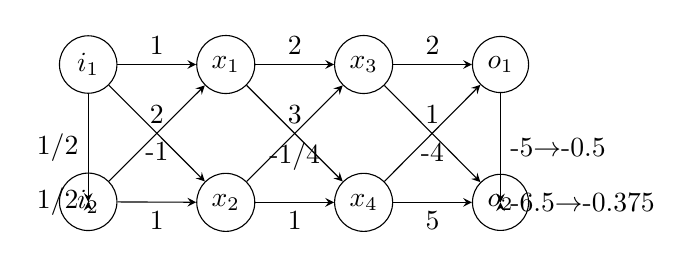
\begin{tikzpicture}[node distance=1cm, auto]
        % Define nodes
        \node [circle, draw] (i1) {$i_{1}$};
        \node [circle, draw, below=of i1] (i2) {$i_{2}$};
        \node [circle, draw, right=of i1] (x1) {$x_{1}$};
        \node [circle, draw, right=of x1] (x3) {$x_{3}$};
        \node [circle, draw, below=of x1] (x2) {$x_{2}$};
        \node [circle, draw, right=of x2] (x4) {$x_{4}$};
        \node [circle, draw, right=of x3] (o1) {$o_{1}$};
        \node [circle, draw, right=of x4] (o2) {$o_{2}$};

        % Draw edges with labels
        \path [-stealth]
            (i1) edge node [above] {1} (x1)
            (i1) edge node [below] {-1} (x2)
            (i2) edge node [above] {2} (x1)
            (i2) edge node [below] {1} (x2)
            (x1) edge node [above] {2} (x3)
            (x1) edge node [below] {-1/4} (x4)
            (x2) edge node [above] {3} (x3)
            (x2) edge node [below] {1} (x4)
            (x3) edge node [above] {2} (o1)
            (x3) edge node [below] {-4} (o2)
            (x4) edge node [above] {1} (o1)
            (x4) edge node [below] {5} (o2)
            (i1) edge node [left] {1/2} (i1 |- i2)
            (i2) edge node [left] {1/2} (i1 |- i2)
            (o1) edge node [right] {-5$\rightarrow$-0.5} (o1 |- o2)
            (o2) edge node [right] {-6.5$\rightarrow$-0.375} (o1 |- o2);
    \end{tikzpicture}
    \caption{Extracted Network}
    \label{fig:extracted_network}
\end{figure}

\end{document}